\documentclass[twoside]{article}
\usepackage{../quiz}
\usepackage{fancyhdr}

\pagestyle{fancy}
\renewcommand{\headrulewidth}{0pt}
\cfoot{}
\rfoot{Solutions at \textbf{\href{http://owenjow.xyz/cs61a/section-quizzes/}{owenjow.xyz/cs61a/section-quizzes}}. Credit to Brian Hou and Kevin Chen for the questions.}
\renewcommand{\footrulewidth}{0.4pt}

\lstset{
    language=Python,
    basicstyle=\ttfamily,
    showstringspaces=false
    keywordstyle=\color{black},
    commentstyle=\color{black},
    stringstyle=\color{black},
    escapeinside={<*}{*>},
}

\def\semester{Spring 2k17}
\newcommand{\solution}[1]{{\color{red}#1}}

%%% Actual, flexible content begins here %%%
\title{\sc Quiz 3 \solution{Solutions}}

\begin{document}
\maketitle

\begin{enumerate}
%%% Q1 %%%
\q{5}{In Shallow Trouble}

Draw the environment diagram that results from executing the code below (until the entire program is finished, or an error occurs).
\vspace{0.1in}

\begin{lstlisting}
def reverse(lst):
    if len(lst) <= 1:
        return lst
    return reverse(lst[1:]) + [lst[0]]

l = [1, [2, 3], 4]
rev = reverse(l)
\end{lstlisting}

\begin{figure}[ht!]
\hspace*{5mm}
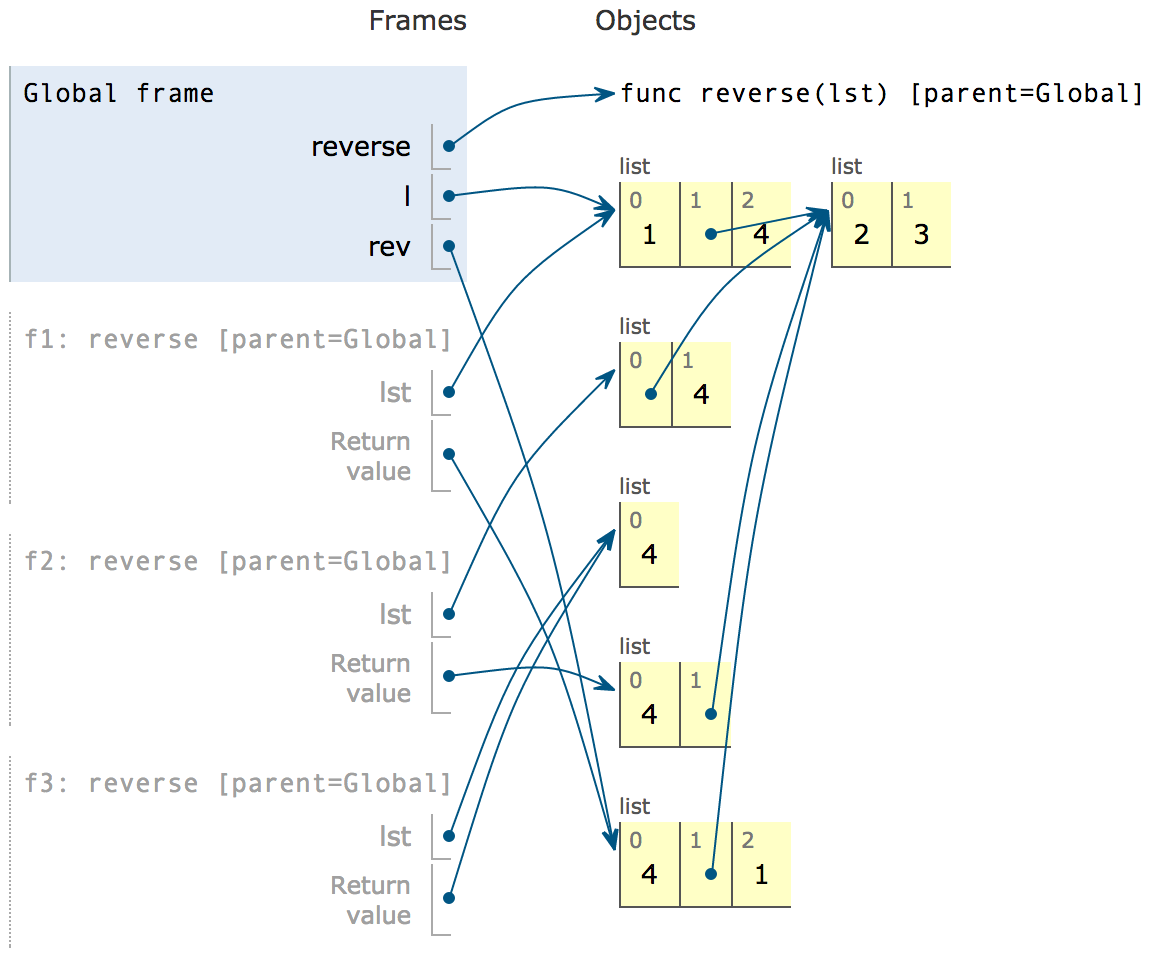
\includegraphics[width=155mm]{../../../../images/quiz3_sol.png}
\end{figure}

\newpage

%%% Q2 %%%
\q{5}{One Three Five One Two}

What does the following code print?
\vspace{0.1in}

\begin{lstlisting}
lst = [None for _ in range(10)]
for i in range(10):
    lst[i] = lambda: i

for func in lst:
    print(func())

<*\solution{9}*>
<*\solution{9}*>
<*\solution{9}*>
<*\solution{9}*>
<*\solution{9}*>
<*\solution{9}*>
<*\solution{9}*>
<*\solution{9}*>
<*\solution{9}*>
<*\solution{9}*>
\end{lstlisting}

\end{enumerate}
\end{document}
